\documentclass[1p]{elsarticle_modified}
%\bibliographystyle{elsarticle-num}

%\usepackage[colorlinks]{hyperref}
%\usepackage{abbrmath_seonhwa} %\Abb, \Ascr, \Acal ,\Abf, \Afrak
\usepackage{amsfonts}
\usepackage{amssymb}
\usepackage{amsmath}
\usepackage{amsthm}
\usepackage{scalefnt}
\usepackage{amsbsy}
\usepackage{kotex}
\usepackage{caption}
\usepackage{subfig}
\usepackage{color}
\usepackage{graphicx}
\usepackage{xcolor} %% white, black, red, green, blue, cyan, magenta, yellow
\usepackage{float}
\usepackage{setspace}
\usepackage{hyperref}

\usepackage{tikz}
\usetikzlibrary{arrows}

\usepackage{multirow}
\usepackage{array} % fixed length table
\usepackage{hhline}

%%%%%%%%%%%%%%%%%%%%%
\makeatletter
\renewcommand*\env@matrix[1][\arraystretch]{%
	\edef\arraystretch{#1}%
	\hskip -\arraycolsep
	\let\@ifnextchar\new@ifnextchar
	\array{*\c@MaxMatrixCols c}}
\makeatother %https://tex.stackexchange.com/questions/14071/how-can-i-increase-the-line-spacing-in-a-matrix
%%%%%%%%%%%%%%%

\usepackage[normalem]{ulem}

\newcommand{\msout}[1]{\ifmmode\text{\sout{\ensuremath{#1}}}\else\sout{#1}\fi}
%SOURCE: \msout is \stkout macro in https://tex.stackexchange.com/questions/20609/strikeout-in-math-mode

\newcommand{\cancel}[1]{
	\ifmmode
	{\color{red}\msout{#1}}
	\else
	{\color{red}\sout{#1}}
	\fi
}

\newcommand{\add}[1]{
	{\color{blue}\uwave{#1}}
}

\newcommand{\replace}[2]{
	\ifmmode
	{\color{red}\msout{#1}}{\color{blue}\uwave{#2}}
	\else
	{\color{red}\sout{#1}}{\color{blue}\uwave{#2}}
	\fi
}

\newcommand{\Sol}{\mathcal{S}} %segment
\newcommand{\D}{D} %diagram
\newcommand{\A}{\mathcal{A}} %arc


%%%%%%%%%%%%%%%%%%%%%%%%%%%%%5 test

\def\sl{\operatorname{\textup{SL}}(2,\Cbb)}
\def\psl{\operatorname{\textup{PSL}}(2,\Cbb)}
\def\quan{\mkern 1mu \triangleright \mkern 1mu}

\theoremstyle{definition}
\newtheorem{thm}{Theorem}[section]
\newtheorem{prop}[thm]{Proposition}
\newtheorem{lem}[thm]{Lemma}
\newtheorem{ques}[thm]{Question}
\newtheorem{cor}[thm]{Corollary}
\newtheorem{defn}[thm]{Definition}
\newtheorem{exam}[thm]{Example}
\newtheorem{rmk}[thm]{Remark}
\newtheorem{alg}[thm]{Algorithm}

\newcommand{\I}{\sqrt{-1}}
\begin{document}

%\begin{frontmatter}
%
%\title{Boundary parabolic representations of knots up to 8 crossings}
%
%%% Group authors per affiliation:
%\author{Yunhi Cho} 
%\address{Department of Mathematics, University of Seoul, Seoul, Korea}
%\ead{yhcho@uos.ac.kr}
%
%
%\author{Seonhwa Kim} %\fnref{s_kim}}
%\address{Center for Geometry and Physics, Institute for Basic Science, Pohang, 37673, Korea}
%\ead{ryeona17@ibs.re.kr}
%
%\author{Hyuk Kim}
%\address{Department of Mathematical Sciences, Seoul National University, Seoul 08826, Korea}
%\ead{hyukkim@snu.ac.kr}
%
%\author{Seokbeom Yoon}
%\address{Department of Mathematical Sciences, Seoul National University, Seoul, 08826,  Korea}
%\ead{sbyoon15@snu.ac.kr}
%
%\begin{abstract}
%We find all boundary parabolic representation of knots up to 8 crossings.
%
%\end{abstract}
%\begin{keyword}
%    \MSC[2010] 57M25 
%\end{keyword}
%
%\end{frontmatter}

%\linenumbers
%\tableofcontents
%
\newcommand\colored[1]{\textcolor{white}{\rule[-0.35ex]{0.8em}{1.4ex}}\kern-0.8em\color{red} #1}%
%\newcommand\colored[1]{\textcolor{white}{ #1}\kern-2.17ex	\textcolor{white}{ #1}\kern-1.81ex	\textcolor{white}{ #1}\kern-2.15ex\color{red}#1	}

{\Large $\underline{12a_{0074}~(K12a_{0074})}$}

\setlength{\tabcolsep}{10pt}
\renewcommand{\arraystretch}{1.6}
\vspace{1cm}\begin{tabular}{m{100pt}>{\centering\arraybackslash}m{274pt}}
\multirow{5}{120pt}{
	\centering
	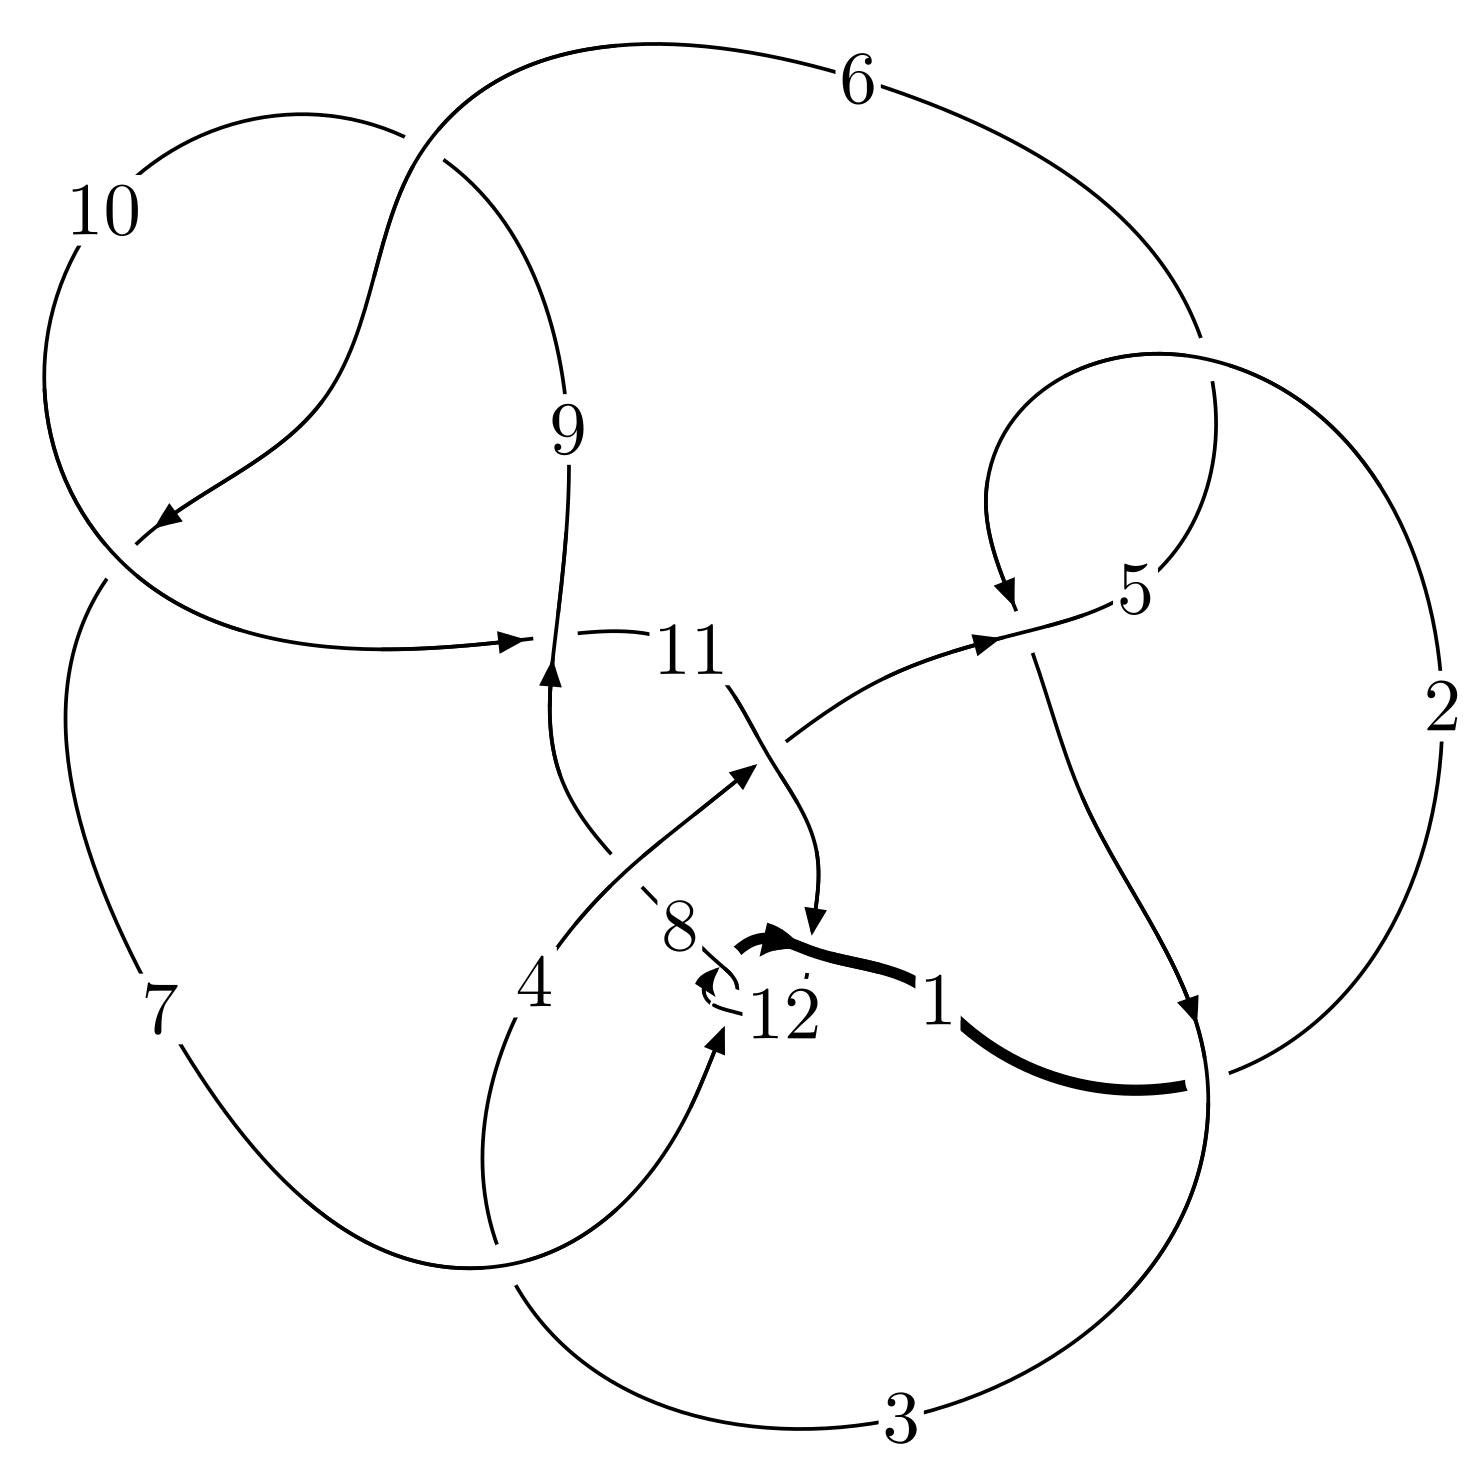
\includegraphics[width=112pt]{../../../GIT/diagram.site/Diagrams/png/875_12a_0074.png}\\
\ \ \ A knot diagram\footnotemark}&
\allowdisplaybreaks
\textbf{Linearized knot diagam} \\
\cline{2-2}
 &
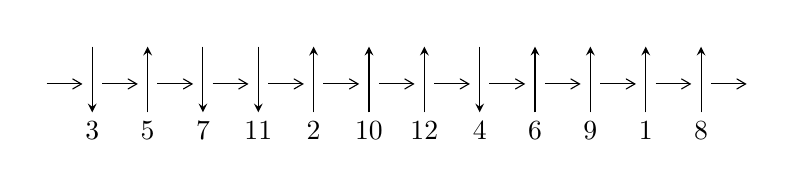
\begin{tikzpicture}[x=20pt, y=17pt]
	% nodes
	\node (C0) at (0, 0) {};
	\node (C1) at (1, 0) {};
	\node (C1U) at (1, +1) {};
	\node (C1D) at (1, -1) {3};

	\node (C2) at (2, 0) {};
	\node (C2U) at (2, +1) {};
	\node (C2D) at (2, -1) {5};

	\node (C3) at (3, 0) {};
	\node (C3U) at (3, +1) {};
	\node (C3D) at (3, -1) {7};

	\node (C4) at (4, 0) {};
	\node (C4U) at (4, +1) {};
	\node (C4D) at (4, -1) {11};

	\node (C5) at (5, 0) {};
	\node (C5U) at (5, +1) {};
	\node (C5D) at (5, -1) {2};

	\node (C6) at (6, 0) {};
	\node (C6U) at (6, +1) {};
	\node (C6D) at (6, -1) {10};

	\node (C7) at (7, 0) {};
	\node (C7U) at (7, +1) {};
	\node (C7D) at (7, -1) {12};

	\node (C8) at (8, 0) {};
	\node (C8U) at (8, +1) {};
	\node (C8D) at (8, -1) {4};

	\node (C9) at (9, 0) {};
	\node (C9U) at (9, +1) {};
	\node (C9D) at (9, -1) {6};

	\node (C10) at (10, 0) {};
	\node (C10U) at (10, +1) {};
	\node (C10D) at (10, -1) {9};

	\node (C11) at (11, 0) {};
	\node (C11U) at (11, +1) {};
	\node (C11D) at (11, -1) {1};

	\node (C12) at (12, 0) {};
	\node (C12U) at (12, +1) {};
	\node (C12D) at (12, -1) {8};
	\node (C13) at (13, 0) {};

	% arrows
	\draw[->,>={angle 60}]
	(C0) edge (C1) (C1) edge (C2) (C2) edge (C3) (C3) edge (C4) (C4) edge (C5) (C5) edge (C6) (C6) edge (C7) (C7) edge (C8) (C8) edge (C9) (C9) edge (C10) (C10) edge (C11) (C11) edge (C12) (C12) edge (C13) ;	\draw[->,>=stealth]
	(C1U) edge (C1D) (C2D) edge (C2U) (C3U) edge (C3D) (C4U) edge (C4D) (C5D) edge (C5U) (C6D) edge (C6U) (C7D) edge (C7U) (C8U) edge (C8D) (C9D) edge (C9U) (C10D) edge (C10U) (C11D) edge (C11U) (C12D) edge (C12U) ;
	\end{tikzpicture} \\
\hhline{~~} \\& 
\textbf{Solving Sequence} \\ \cline{2-2} 
 &
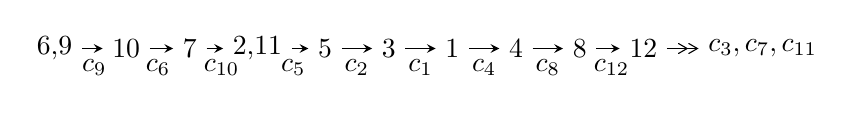
\begin{tikzpicture}[x=23pt, y=7pt]
	% node
	\node (A0) at (-1/8, 0) {6,9};
	\node (A1) at (1, 0) {10};
	\node (A2) at (2, 0) {7};
	\node (A3) at (49/16, 0) {2,11};
	\node (A4) at (33/8, 0) {5};
	\node (A5) at (41/8, 0) {3};
	\node (A6) at (49/8, 0) {1};
	\node (A7) at (57/8, 0) {4};
	\node (A8) at (65/8, 0) {8};
	\node (A9) at (73/8, 0) {12};
	\node (C1) at (1/2, -1) {$c_{9}$};
	\node (C2) at (3/2, -1) {$c_{6}$};
	\node (C3) at (5/2, -1) {$c_{10}$};
	\node (C4) at (29/8, -1) {$c_{5}$};
	\node (C5) at (37/8, -1) {$c_{2}$};
	\node (C6) at (45/8, -1) {$c_{1}$};
	\node (C7) at (53/8, -1) {$c_{4}$};
	\node (C8) at (61/8, -1) {$c_{8}$};
	\node (C9) at (69/8, -1) {$c_{12}$};
	\node (A10) at (11, 0) {$c_{3},c_{7},c_{11}$};

	% edge
	\draw[->,>=stealth]	
	(A0) edge (A1) (A1) edge (A2) (A2) edge (A3) (A3) edge (A4) (A4) edge (A5) (A5) edge (A6) (A6) edge (A7) (A7) edge (A8) (A8) edge (A9) ;
	\draw[->>,>={angle 60}]	
	(A9) edge (A10);
\end{tikzpicture} \\ 

\end{tabular} \\

\footnotetext{
The image of knot diagram is generated by the software ``\textbf{Draw programme}" developed by Andrew Bartholomew(\url{http://www.layer8.co.uk/maths/draw/index.htm\#Running-draw}), where we modified some parts for our purpose(\url{https://github.com/CATsTAILs/LinksPainter}).
}\phantom \\ \newline 
\centering \textbf{Ideals for irreducible components\footnotemark of $X_{\text{par}}$} 
 
\begin{align*}
I^u_{1}&=\langle 
21 u^{30}-29 u^{29}+\cdots+128 b-34,\;-55 u^{30}+76 u^{29}+\cdots+64 a-39,\;u^{31}-2 u^{30}+\cdots+3 u^2+1\rangle \\
I^u_{2}&=\langle 
2.72739\times10^{139} u^{99}+1.28011\times10^{140} u^{98}+\cdots+1.15126\times10^{139} b+3.66899\times10^{139},\\
\phantom{I^u_{2}}&\phantom{= \langle  }-1.38967\times10^{138} u^{99}-9.46861\times10^{138} u^{98}+\cdots+1.15126\times10^{139} a-5.17903\times10^{138},\\
\phantom{I^u_{2}}&\phantom{= \langle  }u^{100}+5 u^{99}+\cdots+2 u+1\rangle \\
I^u_{3}&=\langle 
- a u+2 b+a+2 u,\;a^2+a u+a+u+2,\;u^2+u-1\rangle \\
\\
\end{align*}
\raggedright * 3 irreducible components of $\dim_{\mathbb{C}}=0$, with total 135 representations.\\
\footnotetext{All coefficients of polynomials are rational numbers. But the coefficients are sometimes approximated in decimal forms when there is not enough margin.}
\newpage
\renewcommand{\arraystretch}{1}
\centering \section*{I. $I^u_{1}= \langle 21 u^{30}-29 u^{29}+\cdots+128 b-34,\;-55 u^{30}+76 u^{29}+\cdots+64 a-39,\;u^{31}-2 u^{30}+\cdots+3 u^2+1 \rangle$}
\flushleft \textbf{(i) Arc colorings}\\
\begin{tabular}{m{7pt} m{180pt} m{7pt} m{180pt} }
\flushright $a_{6}=$&$\begin{pmatrix}0\\u\end{pmatrix}$ \\
\flushright $a_{9}=$&$\begin{pmatrix}1\\0\end{pmatrix}$ \\
\flushright $a_{10}=$&$\begin{pmatrix}1\\- u^2\end{pmatrix}$ \\
\flushright $a_{7}=$&$\begin{pmatrix}u\\- u^3+u\end{pmatrix}$ \\
\flushright $a_{2}=$&$\begin{pmatrix}0.859375 u^{30}-1.18750 u^{29}+\cdots+0.750000 u+0.609375\\-0.164063 u^{30}+0.226563 u^{29}+\cdots+1.42969 u+0.265625\end{pmatrix}$ \\
\flushright $a_{11}=$&$\begin{pmatrix}- u^2+1\\- u^2\end{pmatrix}$ \\
\flushright $a_{5}=$&$\begin{pmatrix}\frac{3}{64} u^{30}+\frac{3}{16} u^{29}+\cdots-\frac{9}{8} u+\frac{59}{64}\\-0.335938 u^{30}+0.460938 u^{29}+\cdots+1.25781 u+0.296875\end{pmatrix}$ \\
\flushright $a_{3}=$&$\begin{pmatrix}-0.0781250 u^{30}+0.187500 u^{29}+\cdots+0.375000 u+1.29688\\-0.914063 u^{30}+1.53906 u^{29}+\cdots+1.74219 u+0.453125\end{pmatrix}$ \\
\flushright $a_{1}=$&$\begin{pmatrix}-\frac{1}{2} u^{30}+\frac{1}{2} u^{29}+\cdots+\frac{1}{2} u+1\\-\frac{1}{2} u^{30}+u^{29}+\cdots-4 u^2-\frac{1}{2}\end{pmatrix}$ \\
\flushright $a_{4}=$&$\begin{pmatrix}0.0625000 u^{30}+0.320313 u^{29}+\cdots+0.179688 u+0.867188\\-0.750000 u^{30}+1.31250 u^{29}+\cdots+1.68750 u+0.437500\end{pmatrix}$ \\
\flushright $a_{8}=$&$\begin{pmatrix}\frac{1}{2} u^{30}-\frac{3}{2} u^{29}+\cdots-\frac{1}{2} u^2-\frac{5}{2} u\\\frac{1}{2} u^{30}- u^{29}+\cdots- u-\frac{1}{2}\end{pmatrix}$ \\
\flushright $a_{12}=$&$\begin{pmatrix}-\frac{1}{2} u^{29}+\frac{3}{2} u^{28}+\cdots+\frac{1}{2} u+\frac{3}{2}\\-\frac{1}{2} u^{30}+\frac{1}{2} u^{29}+\cdots-\frac{3}{2} u^2+\frac{1}{2} u\end{pmatrix}$\\&\end{tabular}
\flushleft \textbf{(ii) Obstruction class $= -1$}\\~\\
\flushleft \textbf{(iii) Cusp Shapes $= \frac{159}{128} u^{30}-\frac{693}{256} u^{29}+\cdots+\frac{1725}{256} u+\frac{827}{256}$}\\~\\
\newpage\renewcommand{\arraystretch}{1}
\flushleft \textbf{(iv) u-Polynomials at the component}\newline \\
\begin{tabular}{m{50pt}|m{274pt}}
Crossings & \hspace{64pt}u-Polynomials at each crossing \\
\hline $$\begin{aligned}c_{1}\end{aligned}$$&$\begin{aligned}
&u^{31}+13 u^{30}+\cdots+6432 u-256
\end{aligned}$\\
\hline $$\begin{aligned}c_{2},c_{5}\end{aligned}$$&$\begin{aligned}
&u^{31}- u^{30}+\cdots+88 u+16
\end{aligned}$\\
\hline $$\begin{aligned}c_{3},c_{4}\end{aligned}$$&$\begin{aligned}
&16(16 u^{31}+8 u^{30}+\cdots-4 u^2-1)
\end{aligned}$\\
\hline $$\begin{aligned}c_{6},c_{7},c_{9}\\c_{12}\end{aligned}$$&$\begin{aligned}
&u^{31}+2 u^{30}+\cdots-3 u^2-1
\end{aligned}$\\
\hline $$\begin{aligned}c_{8}\end{aligned}$$&$\begin{aligned}
&u^{31}-5 u^{30}+\cdots+6144 u-1024
\end{aligned}$\\
\hline $$\begin{aligned}c_{10},c_{11}\end{aligned}$$&$\begin{aligned}
&u^{31}-18 u^{30}+\cdots-6 u-1
\end{aligned}$\\
\hline
\end{tabular}\\~\\
\newpage\renewcommand{\arraystretch}{1}
\flushleft \textbf{(v) Riley Polynomials at the component}\newline \\
\begin{tabular}{m{50pt}|m{274pt}}
Crossings & \hspace{64pt}Riley Polynomials at each crossing \\
\hline $$\begin{aligned}c_{1}\end{aligned}$$&$\begin{aligned}
&y^{31}+9 y^{30}+\cdots+52675072 y-65536
\end{aligned}$\\
\hline $$\begin{aligned}c_{2},c_{5}\end{aligned}$$&$\begin{aligned}
&y^{31}+13 y^{30}+\cdots+6432 y-256
\end{aligned}$\\
\hline $$\begin{aligned}c_{3},c_{4}\end{aligned}$$&$\begin{aligned}
&256(256 y^{31}+192 y^{30}+\cdots-8 y-1)
\end{aligned}$\\
\hline $$\begin{aligned}c_{6},c_{7},c_{9}\\c_{12}\end{aligned}$$&$\begin{aligned}
&y^{31}-18 y^{30}+\cdots-6 y-1
\end{aligned}$\\
\hline $$\begin{aligned}c_{8}\end{aligned}$$&$\begin{aligned}
&y^{31}-5 y^{30}+\cdots-7995392 y-1048576
\end{aligned}$\\
\hline $$\begin{aligned}c_{10},c_{11}\end{aligned}$$&$\begin{aligned}
&y^{31}-6 y^{30}+\cdots+122 y-1
\end{aligned}$\\
\hline
\end{tabular}\\~\\
\newpage\flushleft \textbf{(vi) Complex Volumes and Cusp Shapes}
$$\begin{array}{c|c|c}  
\text{Solutions to }I^u_{1}& \I (\text{vol} + \sqrt{-1}CS) & \text{Cusp shape}\\
 \hline 
\begin{aligned}
u &= -0.936680 + 0.338613 I \\
a &= \phantom{-}0.582188 + 1.079190 I \\
b &= \phantom{-}0.048866 + 0.688489 I\end{aligned}
 & \phantom{-}3.50074 - 0.90322 I & \phantom{-}13.05413 + 1.36085 I \\ \hline\begin{aligned}
u &= -0.936680 - 0.338613 I \\
a &= \phantom{-}0.582188 - 1.079190 I \\
b &= \phantom{-}0.048866 - 0.688489 I\end{aligned}
 & \phantom{-}3.50074 + 0.90322 I & \phantom{-}13.05413 - 1.36085 I \\ \hline\begin{aligned}
u &= \phantom{-}0.610112 + 0.779812 I \\
a &= \phantom{-}1.106790 + 0.630784 I \\
b &= \phantom{-}2.03656 - 0.74980 I\end{aligned}
 & -7.60447 + 0.14654 I & -4.01564 - 1.65888 I \\ \hline\begin{aligned}
u &= \phantom{-}0.610112 - 0.779812 I \\
a &= \phantom{-}1.106790 - 0.630784 I \\
b &= \phantom{-}2.03656 + 0.74980 I\end{aligned}
 & -7.60447 - 0.14654 I & -4.01564 + 1.65888 I \\ \hline\begin{aligned}
u &= \phantom{-}0.449445 + 0.919135 I \\
a &= -0.743911 - 1.014000 I \\
b &= -1.45563 + 0.84618 I\end{aligned}
 & -4.77494 - 8.27043 I & -1.01784 + 4.50252 I \\ \hline\begin{aligned}
u &= \phantom{-}0.449445 - 0.919135 I \\
a &= -0.743911 + 1.014000 I \\
b &= -1.45563 - 0.84618 I\end{aligned}
 & -4.77494 + 8.27043 I & -1.01784 - 4.50252 I \\ \hline\begin{aligned}
u &= \phantom{-}0.990236 + 0.401727 I \\
a &= -0.892639 + 0.404991 I \\
b &= -0.264917 + 0.891534 I\end{aligned}
 & \phantom{-}4.39913 + 4.26165 I & \phantom{-}14.5933 - 6.3356 I \\ \hline\begin{aligned}
u &= \phantom{-}0.990236 - 0.401727 I \\
a &= -0.892639 - 0.404991 I \\
b &= -0.264917 - 0.891534 I\end{aligned}
 & \phantom{-}4.39913 - 4.26165 I & \phantom{-}14.5933 + 6.3356 I \\ \hline\begin{aligned}
u &= \phantom{-}0.434243 + 0.819908 I \\
a &= \phantom{-}0.738201 - 0.621086 I \\
b &= \phantom{-}0.265245 - 0.383053 I\end{aligned}
 & -2.40209 - 2.98251 I & \phantom{-}1.29241 + 0.67097 I \\ \hline\begin{aligned}
u &= \phantom{-}0.434243 - 0.819908 I \\
a &= \phantom{-}0.738201 + 0.621086 I \\
b &= \phantom{-}0.265245 + 0.383053 I\end{aligned}
 & -2.40209 + 2.98251 I & \phantom{-}1.29241 - 0.67097 I\\
 \hline 
 \end{array}$$\newpage$$\begin{array}{c|c|c}  
\text{Solutions to }I^u_{1}& \I (\text{vol} + \sqrt{-1}CS) & \text{Cusp shape}\\
 \hline 
\begin{aligned}
u &= -1.002380 + 0.466614 I \\
a &= \phantom{-}1.155680 - 0.270045 I \\
b &= \phantom{-}1.46383 + 0.71776 I\end{aligned}
 & \phantom{-}3.57794 - 7.81275 I & \phantom{-}11.7195 + 11.3359 I \\ \hline\begin{aligned}
u &= -1.002380 - 0.466614 I \\
a &= \phantom{-}1.155680 + 0.270045 I \\
b &= \phantom{-}1.46383 - 0.71776 I\end{aligned}
 & \phantom{-}3.57794 + 7.81275 I & \phantom{-}11.7195 - 11.3359 I \\ \hline\begin{aligned}
u &= \phantom{-}1.005510 + 0.542400 I \\
a &= -1.054370 - 0.734239 I \\
b &= -2.41506 + 1.08769 I\end{aligned}
 & \phantom{-}0.66388 + 10.41550 I & \phantom{-}6.1852 - 13.0772 I \\ \hline\begin{aligned}
u &= \phantom{-}1.005510 - 0.542400 I \\
a &= -1.054370 + 0.734239 I \\
b &= -2.41506 - 1.08769 I\end{aligned}
 & \phantom{-}0.66388 - 10.41550 I & \phantom{-}6.1852 + 13.0772 I \\ \hline\begin{aligned}
u &= \phantom{-}0.766410 + 0.276505 I \\
a &= -0.25730 + 1.48498 I \\
b &= \phantom{-}0.363756 - 0.337678 I\end{aligned}
 & \phantom{-}1.16092 - 1.09032 I & \phantom{-}8.12696 + 0.09273 I \\ \hline\begin{aligned}
u &= \phantom{-}0.766410 - 0.276505 I \\
a &= -0.25730 - 1.48498 I \\
b &= \phantom{-}0.363756 + 0.337678 I\end{aligned}
 & \phantom{-}1.16092 + 1.09032 I & \phantom{-}8.12696 - 0.09273 I \\ \hline\begin{aligned}
u &= -1.021490 + 0.642260 I \\
a &= \phantom{-}0.582856 - 0.986168 I \\
b &= \phantom{-}2.02101 + 0.91098 I\end{aligned}
 & -5.08603 - 10.58260 I & \phantom{-}0.75987 + 9.57565 I \\ \hline\begin{aligned}
u &= -1.021490 - 0.642260 I \\
a &= \phantom{-}0.582856 + 0.986168 I \\
b &= \phantom{-}2.02101 - 0.91098 I\end{aligned}
 & -5.08603 + 10.58260 I & \phantom{-}0.75987 - 9.57565 I \\ \hline\begin{aligned}
u &= -0.579199 + 0.524845 I \\
a &= -0.61005 + 1.48157 I \\
b &= -1.56698 - 0.68703 I\end{aligned}
 & -1.92067 + 1.62049 I & -0.67303 - 1.57224 I \\ \hline\begin{aligned}
u &= -0.579199 - 0.524845 I \\
a &= -0.61005 - 1.48157 I \\
b &= -1.56698 + 0.68703 I\end{aligned}
 & -1.92067 - 1.62049 I & -0.67303 + 1.57224 I\\
 \hline 
 \end{array}$$\newpage$$\begin{array}{c|c|c}  
\text{Solutions to }I^u_{1}& \I (\text{vol} + \sqrt{-1}CS) & \text{Cusp shape}\\
 \hline 
\begin{aligned}
u &= -1.114480 + 0.634528 I \\
a &= -0.496941 - 0.671776 I \\
b &= -0.149359 - 0.970560 I\end{aligned}
 & \phantom{-}1.63726 - 13.87830 I & \phantom{-}6.56033 + 8.55323 I \\ \hline\begin{aligned}
u &= -1.114480 - 0.634528 I \\
a &= -0.496941 + 0.671776 I \\
b &= -0.149359 + 0.970560 I\end{aligned}
 & \phantom{-}1.63726 + 13.87830 I & \phantom{-}6.56033 - 8.55323 I \\ \hline\begin{aligned}
u &= \phantom{-}1.303030 + 0.092850 I \\
a &= \phantom{-}0.555582 + 0.574307 I \\
b &= \phantom{-}1.230900 - 0.232581 I\end{aligned}
 & \phantom{-}8.75635 + 2.55545 I & \phantom{-}15.7194 - 2.3286 I \\ \hline\begin{aligned}
u &= \phantom{-}1.303030 - 0.092850 I \\
a &= \phantom{-}0.555582 - 0.574307 I \\
b &= \phantom{-}1.230900 + 0.232581 I\end{aligned}
 & \phantom{-}8.75635 - 2.55545 I & \phantom{-}15.7194 + 2.3286 I \\ \hline\begin{aligned}
u &= -0.693108\phantom{ +0.000000I} \\
a &= -0.270559\phantom{ +0.000000I} \\
b &= -0.646343\phantom{ +0.000000I}\end{aligned}
 & \phantom{-}1.19574\phantom{ +0.000000I} & \phantom{-}7.87080\phantom{ +0.000000I} \\ \hline\begin{aligned}
u &= -1.134090 + 0.668227 I \\
a &= -0.893764 + 0.503768 I \\
b &= -2.88013 - 0.89189 I\end{aligned}
 & -0.6287 - 19.8896 I & \phantom{-}4.17991 + 11.79937 I \\ \hline\begin{aligned}
u &= -1.134090 - 0.668227 I \\
a &= -0.893764 - 0.503768 I \\
b &= -2.88013 + 0.89189 I\end{aligned}
 & -0.6287 + 19.8896 I & \phantom{-}4.17991 - 11.79937 I \\ \hline\begin{aligned}
u &= \phantom{-}1.60823 + 0.02683 I \\
a &= \phantom{-}0.310056 - 0.550818 I \\
b &= \phantom{-}1.162700 + 0.700629 I\end{aligned}
 & \phantom{-}8.90816 - 2.08408 I & \phantom{-}29.0927 + 62.0574 I \\ \hline\begin{aligned}
u &= \phantom{-}1.60823 - 0.02683 I \\
a &= \phantom{-}0.310056 + 0.550818 I \\
b &= \phantom{-}1.162700 - 0.700629 I\end{aligned}
 & \phantom{-}8.90816 + 2.08408 I & \phantom{-}29.0927 - 62.0574 I \\ \hline\begin{aligned}
u &= -0.032351 + 0.347236 I \\
a &= \phantom{-}2.05290 + 0.96045 I \\
b &= \phantom{-}0.212373 + 0.529053 I\end{aligned}
 & -0.093331 - 1.383200 I & -0.26260 + 4.88905 I\\
 \hline 
 \end{array}$$\newpage$$\begin{array}{c|c|c}  
\text{Solutions to }I^u_{1}& \I (\text{vol} + \sqrt{-1}CS) & \text{Cusp shape}\\
 \hline 
\begin{aligned}
u &= -0.032351 - 0.347236 I \\
a &= \phantom{-}2.05290 - 0.96045 I \\
b &= \phantom{-}0.212373 - 0.529053 I\end{aligned}
 & -0.093331 + 1.383200 I & -0.26260 - 4.88905 I\\
 \hline 
 \end{array}$$\newpage\newpage\renewcommand{\arraystretch}{1}
\centering \section*{II. $I^u_{2}= \langle 2.73\times10^{139} u^{99}+1.28\times10^{140} u^{98}+\cdots+1.15\times10^{139} b+3.67\times10^{139},\;-1.39\times10^{138} u^{99}-9.47\times10^{138} u^{98}+\cdots+1.15\times10^{139} a-5.18\times10^{138},\;u^{100}+5 u^{99}+\cdots+2 u+1 \rangle$}
\flushleft \textbf{(i) Arc colorings}\\
\begin{tabular}{m{7pt} m{180pt} m{7pt} m{180pt} }
\flushright $a_{6}=$&$\begin{pmatrix}0\\u\end{pmatrix}$ \\
\flushright $a_{9}=$&$\begin{pmatrix}1\\0\end{pmatrix}$ \\
\flushright $a_{10}=$&$\begin{pmatrix}1\\- u^2\end{pmatrix}$ \\
\flushright $a_{7}=$&$\begin{pmatrix}u\\- u^3+u\end{pmatrix}$ \\
\flushright $a_{2}=$&$\begin{pmatrix}0.120709 u^{99}+0.822455 u^{98}+\cdots+2.52213 u+0.449857\\-2.36904 u^{99}-11.1192 u^{98}+\cdots-0.977338 u-3.18693\end{pmatrix}$ \\
\flushright $a_{11}=$&$\begin{pmatrix}- u^2+1\\- u^2\end{pmatrix}$ \\
\flushright $a_{5}=$&$\begin{pmatrix}-0.488022 u^{99}-2.16943 u^{98}+\cdots+3.31259 u-0.818863\\-2.16817 u^{99}-9.37783 u^{98}+\cdots-0.240999 u-1.66392\end{pmatrix}$ \\
\flushright $a_{3}=$&$\begin{pmatrix}-0.373898 u^{99}-1.57574 u^{98}+\cdots+5.49285 u-0.603726\\-2.25516 u^{99}-9.47053 u^{98}+\cdots-0.392895 u-1.57015\end{pmatrix}$ \\
\flushright $a_{1}=$&$\begin{pmatrix}0.0996443 u^{99}-0.000163284 u^{98}+\cdots-0.496826 u-0.698151\\-0.844919 u^{99}-4.49402 u^{98}+\cdots-2.62234 u-2.17334\end{pmatrix}$ \\
\flushright $a_{4}=$&$\begin{pmatrix}0.308833 u^{99}+2.43088 u^{98}+\cdots+6.45605 u+0.901556\\0.332759 u^{99}+1.55082 u^{98}+\cdots+2.43896 u+0.528091\end{pmatrix}$ \\
\flushright $a_{8}=$&$\begin{pmatrix}2.17334 u^{99}+10.0218 u^{98}+\cdots+3.43426 u+1.72433\\0.498385 u^{99}+1.78125 u^{98}+\cdots+0.897440 u+0.0996443\end{pmatrix}$ \\
\flushright $a_{12}=$&$\begin{pmatrix}-0.904282 u^{99}-4.89024 u^{98}+\cdots-4.39589 u-0.802382\\-1.62929 u^{99}-7.37061 u^{98}+\cdots-4.26428 u-1.54217\end{pmatrix}$\\&\end{tabular}
\flushleft \textbf{(ii) Obstruction class $= -1$}\\~\\
\flushleft \textbf{(iii) Cusp Shapes $= -5.53328 u^{99}-25.3817 u^{98}+\cdots-11.0157 u-1.28022$}\\~\\
\newpage\renewcommand{\arraystretch}{1}
\flushleft \textbf{(iv) u-Polynomials at the component}\newline \\
\begin{tabular}{m{50pt}|m{274pt}}
Crossings & \hspace{64pt}u-Polynomials at each crossing \\
\hline $$\begin{aligned}c_{1}\end{aligned}$$&$\begin{aligned}
&(u^{50}+22 u^{49}+\cdots-26 u+1)^{2}
\end{aligned}$\\
\hline $$\begin{aligned}c_{2},c_{5}\end{aligned}$$&$\begin{aligned}
&(u^{50}+2 u^{49}+\cdots+10 u+1)^{2}
\end{aligned}$\\
\hline $$\begin{aligned}c_{3},c_{4}\end{aligned}$$&$\begin{aligned}
&u^{100}+7 u^{99}+\cdots+1086100 u+143123
\end{aligned}$\\
\hline $$\begin{aligned}c_{6},c_{7},c_{9}\\c_{12}\end{aligned}$$&$\begin{aligned}
&u^{100}-5 u^{99}+\cdots-2 u+1
\end{aligned}$\\
\hline $$\begin{aligned}c_{8}\end{aligned}$$&$\begin{aligned}
&(u^{50}+2 u^{49}+\cdots+4 u+1)^{2}
\end{aligned}$\\
\hline $$\begin{aligned}c_{10},c_{11}\end{aligned}$$&$\begin{aligned}
&u^{100}-41 u^{99}+\cdots+30 u^2+1
\end{aligned}$\\
\hline
\end{tabular}\\~\\
\newpage\renewcommand{\arraystretch}{1}
\flushleft \textbf{(v) Riley Polynomials at the component}\newline \\
\begin{tabular}{m{50pt}|m{274pt}}
Crossings & \hspace{64pt}Riley Polynomials at each crossing \\
\hline $$\begin{aligned}c_{1}\end{aligned}$$&$\begin{aligned}
&(y^{50}+14 y^{49}+\cdots-1050 y+1)^{2}
\end{aligned}$\\
\hline $$\begin{aligned}c_{2},c_{5}\end{aligned}$$&$\begin{aligned}
&(y^{50}+22 y^{49}+\cdots-26 y+1)^{2}
\end{aligned}$\\
\hline $$\begin{aligned}c_{3},c_{4}\end{aligned}$$&$\begin{aligned}
&y^{100}-33 y^{99}+\cdots+855156748636 y+20484193129
\end{aligned}$\\
\hline $$\begin{aligned}c_{6},c_{7},c_{9}\\c_{12}\end{aligned}$$&$\begin{aligned}
&y^{100}-41 y^{99}+\cdots+30 y^2+1
\end{aligned}$\\
\hline $$\begin{aligned}c_{8}\end{aligned}$$&$\begin{aligned}
&(y^{50}-10 y^{49}+\cdots+10 y+1)^{2}
\end{aligned}$\\
\hline $$\begin{aligned}c_{10},c_{11}\end{aligned}$$&$\begin{aligned}
&y^{100}+35 y^{99}+\cdots+60 y+1
\end{aligned}$\\
\hline
\end{tabular}\\~\\
\newpage\flushleft \textbf{(vi) Complex Volumes and Cusp Shapes}
$$\begin{array}{c|c|c}  
\text{Solutions to }I^u_{2}& \I (\text{vol} + \sqrt{-1}CS) & \text{Cusp shape}\\
 \hline 
\begin{aligned}
u &= \phantom{-}0.805392 + 0.565666 I \\
a &= \phantom{-}0.137398 + 0.910966 I \\
b &= \phantom{-}3.71411 - 1.57836 I\end{aligned}
 & -0.21807 + 2.45541 I & \phantom{-0.000000 } 0 \\ \hline\begin{aligned}
u &= \phantom{-}0.805392 - 0.565666 I \\
a &= \phantom{-}0.137398 - 0.910966 I \\
b &= \phantom{-}3.71411 + 1.57836 I\end{aligned}
 & -0.21807 - 2.45541 I & \phantom{-0.000000 } 0 \\ \hline\begin{aligned}
u &= \phantom{-}0.870372 + 0.532948 I \\
a &= -0.844290 - 0.471246 I \\
b &= -4.88150 + 8.11072 I\end{aligned}
 & -0.03678 + 1.97726 I & \phantom{-0.000000 } 0 \\ \hline\begin{aligned}
u &= \phantom{-}0.870372 - 0.532948 I \\
a &= -0.844290 + 0.471246 I \\
b &= -4.88150 - 8.11072 I\end{aligned}
 & -0.03678 - 1.97726 I & \phantom{-0.000000 } 0 \\ \hline\begin{aligned}
u &= \phantom{-}0.897882 + 0.487726 I \\
a &= -0.014174 + 0.965644 I \\
b &= -1.09023 + 8.22715 I\end{aligned}
 & -0.03678 - 1.97726 I & \phantom{-0.000000 } 0 \\ \hline\begin{aligned}
u &= \phantom{-}0.897882 - 0.487726 I \\
a &= -0.014174 - 0.965644 I \\
b &= -1.09023 - 8.22715 I\end{aligned}
 & -0.03678 + 1.97726 I & \phantom{-0.000000 } 0 \\ \hline\begin{aligned}
u &= -0.464448 + 0.914988 I \\
a &= \phantom{-}0.718491 - 1.066280 I \\
b &= \phantom{-}1.50650 + 0.81554 I\end{aligned}
 & -2.6715 + 14.0778 I & \phantom{-0.000000 } 0 \\ \hline\begin{aligned}
u &= -0.464448 - 0.914988 I \\
a &= \phantom{-}0.718491 + 1.066280 I \\
b &= \phantom{-}1.50650 - 0.81554 I\end{aligned}
 & -2.6715 - 14.0778 I & \phantom{-0.000000 } 0 \\ \hline\begin{aligned}
u &= \phantom{-}0.345540 + 0.905171 I \\
a &= -0.888803 - 0.791753 I \\
b &= -1.21930 + 0.92283 I\end{aligned}
 & -5.90869 - 3.57059 I & \phantom{-0.000000 } 0 \\ \hline\begin{aligned}
u &= \phantom{-}0.345540 - 0.905171 I \\
a &= -0.888803 + 0.791753 I \\
b &= -1.21930 - 0.92283 I\end{aligned}
 & -5.90869 + 3.57059 I & \phantom{-0.000000 } 0\\
 \hline 
 \end{array}$$\newpage$$\begin{array}{c|c|c}  
\text{Solutions to }I^u_{2}& \I (\text{vol} + \sqrt{-1}CS) & \text{Cusp shape}\\
 \hline 
\begin{aligned}
u &= -0.599800 + 0.750932 I \\
a &= -0.150280 - 0.616290 I \\
b &= \phantom{-}0.303124 + 0.349454 I\end{aligned}
 & -1.29692 - 5.01538 I & \phantom{-0.000000 } 0 \\ \hline\begin{aligned}
u &= -0.599800 - 0.750932 I \\
a &= -0.150280 + 0.616290 I \\
b &= \phantom{-}0.303124 - 0.349454 I\end{aligned}
 & -1.29692 + 5.01538 I & \phantom{-0.000000 } 0 \\ \hline\begin{aligned}
u &= -0.592726 + 0.753085 I \\
a &= -1.139510 + 0.755454 I \\
b &= -2.06616 - 0.74386 I\end{aligned}
 & -6.37316 + 5.28105 I & \phantom{-0.000000 } 0 \\ \hline\begin{aligned}
u &= -0.592726 - 0.753085 I \\
a &= -1.139510 - 0.755454 I \\
b &= -2.06616 + 0.74386 I\end{aligned}
 & -6.37316 - 5.28105 I & \phantom{-0.000000 } 0 \\ \hline\begin{aligned}
u &= \phantom{-}0.995575 + 0.307242 I \\
a &= -0.329780 - 0.755301 I \\
b &= \phantom{-}0.892626 - 0.159113 I\end{aligned}
 & -0.59812 + 5.40527 I & \phantom{-0.000000 } 0 \\ \hline\begin{aligned}
u &= \phantom{-}0.995575 - 0.307242 I \\
a &= -0.329780 + 0.755301 I \\
b &= \phantom{-}0.892626 + 0.159113 I\end{aligned}
 & -0.59812 - 5.40527 I & \phantom{-0.000000 } 0 \\ \hline\begin{aligned}
u &= -0.963434 + 0.399072 I \\
a &= \phantom{-}0.512485 + 0.510292 I \\
b &= -0.011941 + 0.888950 I\end{aligned}
 & \phantom{-}2.04137 - 1.36627 I & \phantom{-0.000000 } 0 \\ \hline\begin{aligned}
u &= -0.963434 - 0.399072 I \\
a &= \phantom{-}0.512485 - 0.510292 I \\
b &= -0.011941 - 0.888950 I\end{aligned}
 & \phantom{-}2.04137 + 1.36627 I & \phantom{-0.000000 } 0 \\ \hline\begin{aligned}
u &= \phantom{-}0.975907 + 0.372400 I \\
a &= -0.772650 + 0.760018 I \\
b &= -0.069798 + 0.950611 I\end{aligned}
 & \phantom{-}4.18629 - 1.80724 I & \phantom{-0.000000 } 0 \\ \hline\begin{aligned}
u &= \phantom{-}0.975907 - 0.372400 I \\
a &= -0.772650 - 0.760018 I \\
b &= -0.069798 - 0.950611 I\end{aligned}
 & \phantom{-}4.18629 + 1.80724 I & \phantom{-0.000000 } 0\\
 \hline 
 \end{array}$$\newpage$$\begin{array}{c|c|c}  
\text{Solutions to }I^u_{2}& \I (\text{vol} + \sqrt{-1}CS) & \text{Cusp shape}\\
 \hline 
\begin{aligned}
u &= -0.941662 + 0.467528 I \\
a &= \phantom{-}0.001522 + 0.862430 I \\
b &= -0.70376 + 3.30787 I\end{aligned}
 & -0.21807 - 2.45541 I & \phantom{-0.000000 } 0 \\ \hline\begin{aligned}
u &= -0.941662 - 0.467528 I \\
a &= \phantom{-}0.001522 - 0.862430 I \\
b &= -0.70376 - 3.30787 I\end{aligned}
 & -0.21807 + 2.45541 I & \phantom{-0.000000 } 0 \\ \hline\begin{aligned}
u &= -0.438799 + 0.840334 I \\
a &= -0.815677 - 0.656198 I \\
b &= -0.308347 - 0.529533 I\end{aligned}
 & -0.38497 + 8.39332 I & \phantom{-0.000000 } 0 \\ \hline\begin{aligned}
u &= -0.438799 - 0.840334 I \\
a &= -0.815677 + 0.656198 I \\
b &= -0.308347 + 0.529533 I\end{aligned}
 & -0.38497 - 8.39332 I & \phantom{-0.000000 } 0 \\ \hline\begin{aligned}
u &= -0.895331 + 0.277953 I \\
a &= \phantom{-}0.49067 + 1.34070 I \\
b &= -0.213926 + 0.271473 I\end{aligned}
 & \phantom{-}2.41061 + 4.79603 I & \phantom{-0.000000 } 0 \\ \hline\begin{aligned}
u &= -0.895331 - 0.277953 I \\
a &= \phantom{-}0.49067 - 1.34070 I \\
b &= -0.213926 - 0.271473 I\end{aligned}
 & \phantom{-}2.41061 - 4.79603 I & \phantom{-0.000000 } 0 \\ \hline\begin{aligned}
u &= -0.452534 + 0.971496 I \\
a &= \phantom{-}0.638057 - 0.904792 I \\
b &= \phantom{-}1.35669 + 0.76688 I\end{aligned}
 & \phantom{-}1.58339 + 5.46834 I & \phantom{-0.000000 } 0 \\ \hline\begin{aligned}
u &= -0.452534 - 0.971496 I \\
a &= \phantom{-}0.638057 + 0.904792 I \\
b &= \phantom{-}1.35669 - 0.76688 I\end{aligned}
 & \phantom{-}1.58339 - 5.46834 I & \phantom{-0.000000 } 0 \\ \hline\begin{aligned}
u &= -0.362849 + 0.852585 I \\
a &= -0.821536 - 0.441844 I \\
b &= -0.638247 - 0.245214 I\end{aligned}
 & \phantom{-}3.03278 + 0.55194 I & \phantom{-0.000000 } 0 \\ \hline\begin{aligned}
u &= -0.362849 - 0.852585 I \\
a &= -0.821536 + 0.441844 I \\
b &= -0.638247 + 0.245214 I\end{aligned}
 & \phantom{-}3.03278 - 0.55194 I & \phantom{-0.000000 } 0\\
 \hline 
 \end{array}$$\newpage$$\begin{array}{c|c|c}  
\text{Solutions to }I^u_{2}& \I (\text{vol} + \sqrt{-1}CS) & \text{Cusp shape}\\
 \hline 
\begin{aligned}
u &= \phantom{-}0.972507 + 0.459567 I \\
a &= -0.932367 - 0.289538 I \\
b &= -1.320190 - 0.016880 I\end{aligned}
 & \phantom{-}1.69220 + 4.35370 I & \phantom{-0.000000 } 0 \\ \hline\begin{aligned}
u &= \phantom{-}0.972507 - 0.459567 I \\
a &= -0.932367 + 0.289538 I \\
b &= -1.320190 + 0.016880 I\end{aligned}
 & \phantom{-}1.69220 - 4.35370 I & \phantom{-0.000000 } 0 \\ \hline\begin{aligned}
u &= \phantom{-}0.845214 + 0.350717 I \\
a &= -0.269449 + 1.229150 I \\
b &= -0.360530 - 0.128486 I\end{aligned}
 & \phantom{-}0.96274 - 1.04006 I & \phantom{-0.000000 } 0 \\ \hline\begin{aligned}
u &= \phantom{-}0.845214 - 0.350717 I \\
a &= -0.269449 - 1.229150 I \\
b &= -0.360530 + 0.128486 I\end{aligned}
 & \phantom{-}0.96274 + 1.04006 I & \phantom{-0.000000 } 0 \\ \hline\begin{aligned}
u &= -0.996807 + 0.435728 I \\
a &= \phantom{-}1.040630 - 0.000544 I \\
b &= \phantom{-}0.811839 + 0.685261 I\end{aligned}
 & \phantom{-}4.18629 - 1.80724 I & \phantom{-0.000000 } 0 \\ \hline\begin{aligned}
u &= -0.996807 - 0.435728 I \\
a &= \phantom{-}1.040630 + 0.000544 I \\
b &= \phantom{-}0.811839 - 0.685261 I\end{aligned}
 & \phantom{-}4.18629 + 1.80724 I & \phantom{-0.000000 } 0 \\ \hline\begin{aligned}
u &= -0.940675 + 0.571103 I \\
a &= \phantom{-}0.797850 - 0.614339 I \\
b &= \phantom{-}2.78678 + 1.76470 I\end{aligned}
 & -0.74785 - 5.64906 I & \phantom{-0.000000 } 0 \\ \hline\begin{aligned}
u &= -0.940675 - 0.571103 I \\
a &= \phantom{-}0.797850 + 0.614339 I \\
b &= \phantom{-}2.78678 - 1.76470 I\end{aligned}
 & -0.74785 + 5.64906 I & \phantom{-0.000000 } 0 \\ \hline\begin{aligned}
u &= \phantom{-}0.640859 + 0.895863 I \\
a &= \phantom{-}1.012390 + 0.267051 I \\
b &= \phantom{-}1.88350 - 0.68017 I\end{aligned}
 & -5.90869 + 3.57059 I & \phantom{-0.000000 } 0 \\ \hline\begin{aligned}
u &= \phantom{-}0.640859 - 0.895863 I \\
a &= \phantom{-}1.012390 - 0.267051 I \\
b &= \phantom{-}1.88350 + 0.68017 I\end{aligned}
 & -5.90869 - 3.57059 I & \phantom{-0.000000 } 0\\
 \hline 
 \end{array}$$\newpage$$\begin{array}{c|c|c}  
\text{Solutions to }I^u_{2}& \I (\text{vol} + \sqrt{-1}CS) & \text{Cusp shape}\\
 \hline 
\begin{aligned}
u &= -0.704941 + 0.555049 I \\
a &= -0.390234 + 1.107560 I \\
b &= -1.92721 - 1.30059 I\end{aligned}
 & -1.47932 + 1.10651 I & \phantom{-0.000000 } 0 \\ \hline\begin{aligned}
u &= -0.704941 - 0.555049 I \\
a &= -0.390234 - 1.107560 I \\
b &= -1.92721 + 1.30059 I\end{aligned}
 & -1.47932 - 1.10651 I & \phantom{-0.000000 } 0 \\ \hline\begin{aligned}
u &= -0.958259 + 0.559233 I \\
a &= -0.136771 - 0.079819 I \\
b &= -1.065870 + 0.002940 I\end{aligned}
 & -0.223424\phantom{ +0.000000I} & \phantom{-0.000000 } 0 \\ \hline\begin{aligned}
u &= -0.958259 - 0.559233 I \\
a &= -0.136771 + 0.079819 I \\
b &= -1.065870 - 0.002940 I\end{aligned}
 & -0.223424\phantom{ +0.000000I} & \phantom{-0.000000 } 0 \\ \hline\begin{aligned}
u &= -0.287367 + 0.842417 I \\
a &= \phantom{-}1.009560 - 0.693922 I \\
b &= \phantom{-}1.04412 + 0.95613 I\end{aligned}
 & -4.78948 - 2.42792 I & \phantom{-0.000000 } 0 \\ \hline\begin{aligned}
u &= -0.287367 - 0.842417 I \\
a &= \phantom{-}1.009560 + 0.693922 I \\
b &= \phantom{-}1.04412 - 0.95613 I\end{aligned}
 & -4.78948 + 2.42792 I & \phantom{-0.000000 } 0 \\ \hline\begin{aligned}
u &= -0.900705 + 0.652680 I \\
a &= \phantom{-}0.520199 - 0.570395 I \\
b &= \phantom{-}1.27971 + 1.85358 I\end{aligned}
 & -0.59812 - 5.40527 I & \phantom{-0.000000 } 0 \\ \hline\begin{aligned}
u &= -0.900705 - 0.652680 I \\
a &= \phantom{-}0.520199 + 0.570395 I \\
b &= \phantom{-}1.27971 - 1.85358 I\end{aligned}
 & -0.59812 + 5.40527 I & \phantom{-0.000000 } 0 \\ \hline\begin{aligned}
u &= \phantom{-}0.508428 + 0.727312 I \\
a &= \phantom{-}0.383289 - 0.548299 I \\
b &= -0.0213567 + 0.1030520 I\end{aligned}
 & -3.00190\phantom{ +0.000000I} & \phantom{-0.000000 } 0 \\ \hline\begin{aligned}
u &= \phantom{-}0.508428 - 0.727312 I \\
a &= \phantom{-}0.383289 + 0.548299 I \\
b &= -0.0213567 - 0.1030520 I\end{aligned}
 & -3.00190\phantom{ +0.000000I} & \phantom{-0.000000 } 0\\
 \hline 
 \end{array}$$\newpage$$\begin{array}{c|c|c}  
\text{Solutions to }I^u_{2}& \I (\text{vol} + \sqrt{-1}CS) & \text{Cusp shape}\\
 \hline 
\begin{aligned}
u &= \phantom{-}0.992128 + 0.505162 I \\
a &= -1.083540 - 0.520726 I \\
b &= -2.20138 + 0.72198 I\end{aligned}
 & \phantom{-}2.41061 + 4.79603 I & \phantom{-0.000000 } 0 \\ \hline\begin{aligned}
u &= \phantom{-}0.992128 - 0.505162 I \\
a &= -1.083540 + 0.520726 I \\
b &= -2.20138 - 0.72198 I\end{aligned}
 & \phantom{-}2.41061 - 4.79603 I & \phantom{-0.000000 } 0 \\ \hline\begin{aligned}
u &= -0.597441 + 0.939870 I \\
a &= -1.052590 + 0.123829 I \\
b &= -1.76623 - 0.67472 I\end{aligned}
 & -3.40724 - 9.26124 I & \phantom{-0.000000 } 0 \\ \hline\begin{aligned}
u &= -0.597441 - 0.939870 I \\
a &= -1.052590 - 0.123829 I \\
b &= -1.76623 + 0.67472 I\end{aligned}
 & -3.40724 + 9.26124 I & \phantom{-0.000000 } 0 \\ \hline\begin{aligned}
u &= -0.985911 + 0.554260 I \\
a &= \phantom{-}0.941721 - 0.708633 I \\
b &= \phantom{-}2.53950 + 1.14071 I\end{aligned}
 & -0.73924 - 6.06918 I & \phantom{-0.000000 } 0 \\ \hline\begin{aligned}
u &= -0.985911 - 0.554260 I \\
a &= \phantom{-}0.941721 + 0.708633 I \\
b &= \phantom{-}2.53950 - 1.14071 I\end{aligned}
 & -0.73924 + 6.06918 I & \phantom{-0.000000 } 0 \\ \hline\begin{aligned}
u &= -0.804423 + 0.810841 I \\
a &= -0.683704 + 0.364209 I \\
b &= -2.01847 - 0.56368 I\end{aligned}
 & -0.915526 - 0.076578 I & \phantom{-0.000000 } 0 \\ \hline\begin{aligned}
u &= -0.804423 - 0.810841 I \\
a &= -0.683704 - 0.364209 I \\
b &= -2.01847 + 0.56368 I\end{aligned}
 & -0.915526 + 0.076578 I & \phantom{-0.000000 } 0 \\ \hline\begin{aligned}
u &= -1.196350 + 0.125224 I \\
a &= -0.604684 + 0.388170 I \\
b &= -1.214590 - 0.044805 I\end{aligned}
 & \phantom{-}3.03278 + 0.55194 I & \phantom{-0.000000 } 0 \\ \hline\begin{aligned}
u &= -1.196350 - 0.125224 I \\
a &= -0.604684 - 0.388170 I \\
b &= -1.214590 + 0.044805 I\end{aligned}
 & \phantom{-}3.03278 - 0.55194 I & \phantom{-0.000000 } 0\\
 \hline 
 \end{array}$$\newpage$$\begin{array}{c|c|c}  
\text{Solutions to }I^u_{2}& \I (\text{vol} + \sqrt{-1}CS) & \text{Cusp shape}\\
 \hline 
\begin{aligned}
u &= \phantom{-}1.205060 + 0.085428 I \\
a &= \phantom{-}0.703335 + 0.405377 I \\
b &= \phantom{-}1.157630 - 0.080797 I\end{aligned}
 & \phantom{-}5.29694 - 5.97751 I & \phantom{-0.000000 } 0 \\ \hline\begin{aligned}
u &= \phantom{-}1.205060 - 0.085428 I \\
a &= \phantom{-}0.703335 - 0.405377 I \\
b &= \phantom{-}1.157630 + 0.080797 I\end{aligned}
 & \phantom{-}5.29694 + 5.97751 I & \phantom{-0.000000 } 0 \\ \hline\begin{aligned}
u &= \phantom{-}1.017910 + 0.659027 I \\
a &= -0.511569 - 0.951740 I \\
b &= -1.86748 + 0.89291 I\end{aligned}
 & -6.37316 + 5.28105 I & \phantom{-0.000000 } 0 \\ \hline\begin{aligned}
u &= \phantom{-}1.017910 - 0.659027 I \\
a &= -0.511569 + 0.951740 I \\
b &= -1.86748 - 0.89291 I\end{aligned}
 & -6.37316 - 5.28105 I & \phantom{-0.000000 } 0 \\ \hline\begin{aligned}
u &= -1.174210 + 0.323836 I \\
a &= -0.016603 - 0.726219 I \\
b &= -0.723369 + 0.106438 I\end{aligned}
 & -0.915526 + 0.076578 I & \phantom{-0.000000 } 0 \\ \hline\begin{aligned}
u &= -1.174210 - 0.323836 I \\
a &= -0.016603 + 0.726219 I \\
b &= -0.723369 - 0.106438 I\end{aligned}
 & -0.915526 - 0.076578 I & \phantom{-0.000000 } 0 \\ \hline\begin{aligned}
u &= \phantom{-}1.073530 + 0.580651 I \\
a &= \phantom{-}0.298381 - 0.400600 I \\
b &= \phantom{-}0.662813 - 0.460597 I\end{aligned}
 & -1.29692 + 5.01538 I & \phantom{-0.000000 } 0 \\ \hline\begin{aligned}
u &= \phantom{-}1.073530 - 0.580651 I \\
a &= \phantom{-}0.298381 + 0.400600 I \\
b &= \phantom{-}0.662813 + 0.460597 I\end{aligned}
 & -1.29692 - 5.01538 I & \phantom{-0.000000 } 0 \\ \hline\begin{aligned}
u &= \phantom{-}1.009330 + 0.740780 I \\
a &= -0.306559 - 0.815188 I \\
b &= -1.29785 + 0.84084 I\end{aligned}
 & -4.78948 + 2.42792 I & \phantom{-0.000000 } 0 \\ \hline\begin{aligned}
u &= \phantom{-}1.009330 - 0.740780 I \\
a &= -0.306559 + 0.815188 I \\
b &= -1.29785 - 0.84084 I\end{aligned}
 & -4.78948 - 2.42792 I & \phantom{-0.000000 } 0\\
 \hline 
 \end{array}$$\newpage$$\begin{array}{c|c|c}  
\text{Solutions to }I^u_{2}& \I (\text{vol} + \sqrt{-1}CS) & \text{Cusp shape}\\
 \hline 
\begin{aligned}
u &= \phantom{-}1.111390 + 0.627622 I \\
a &= \phantom{-}0.467225 - 0.621515 I \\
b &= \phantom{-}0.250207 - 0.878108 I\end{aligned}
 & -0.38497 + 8.39332 I & \phantom{-0.000000 } 0 \\ \hline\begin{aligned}
u &= \phantom{-}1.111390 - 0.627622 I \\
a &= \phantom{-}0.467225 + 0.621515 I \\
b &= \phantom{-}0.250207 + 0.878108 I\end{aligned}
 & -0.38497 - 8.39332 I & \phantom{-0.000000 } 0 \\ \hline\begin{aligned}
u &= \phantom{-}1.279170 + 0.025724 I \\
a &= \phantom{-}0.491611 - 0.840663 I \\
b &= \phantom{-}1.073100 + 0.269183 I\end{aligned}
 & \phantom{-}3.73617 - 11.46140 I & \phantom{-0.000000 } 0 \\ \hline\begin{aligned}
u &= \phantom{-}1.279170 - 0.025724 I \\
a &= \phantom{-}0.491611 + 0.840663 I \\
b &= \phantom{-}1.073100 - 0.269183 I\end{aligned}
 & \phantom{-}3.73617 + 11.46140 I & \phantom{-0.000000 } 0 \\ \hline\begin{aligned}
u &= -1.132260 + 0.619924 I \\
a &= -0.348291 - 0.675201 I \\
b &= -0.074295 - 0.616385 I\end{aligned}
 & \phantom{-}5.29694 - 5.97751 I & \phantom{-0.000000 } 0 \\ \hline\begin{aligned}
u &= -1.132260 - 0.619924 I \\
a &= -0.348291 + 0.675201 I \\
b &= -0.074295 + 0.616385 I\end{aligned}
 & \phantom{-}5.29694 + 5.97751 I & \phantom{-0.000000 } 0 \\ \hline\begin{aligned}
u &= \phantom{-}0.502314 + 0.490863 I \\
a &= \phantom{-}0.66915 + 1.77608 I \\
b &= \phantom{-}1.45721 - 0.37222 I\end{aligned}
 & -0.73924 - 6.06918 I & \phantom{-}2.41006 + 7.32858 I \\ \hline\begin{aligned}
u &= \phantom{-}0.502314 - 0.490863 I \\
a &= \phantom{-}0.66915 - 1.77608 I \\
b &= \phantom{-}1.45721 + 0.37222 I\end{aligned}
 & -0.73924 + 6.06918 I & \phantom{-}2.41006 - 7.32858 I \\ \hline\begin{aligned}
u &= -1.302470 + 0.047049 I \\
a &= -0.424085 - 0.805603 I \\
b &= -1.056750 + 0.299631 I\end{aligned}
 & \phantom{-}1.58339 + 5.46834 I & \phantom{-0.000000 } 0 \\ \hline\begin{aligned}
u &= -1.302470 - 0.047049 I \\
a &= -0.424085 + 0.805603 I \\
b &= -1.056750 - 0.299631 I\end{aligned}
 & \phantom{-}1.58339 - 5.46834 I & \phantom{-0.000000 } 0\\
 \hline 
 \end{array}$$\newpage$$\begin{array}{c|c|c}  
\text{Solutions to }I^u_{2}& \I (\text{vol} + \sqrt{-1}CS) & \text{Cusp shape}\\
 \hline 
\begin{aligned}
u &= \phantom{-}1.140050 + 0.665009 I \\
a &= \phantom{-}0.860159 + 0.509302 I \\
b &= \phantom{-}2.85078 - 0.81091 I\end{aligned}
 & -2.6715 + 14.0778 I & \phantom{-0.000000 } 0 \\ \hline\begin{aligned}
u &= \phantom{-}1.140050 - 0.665009 I \\
a &= \phantom{-}0.860159 - 0.509302 I \\
b &= \phantom{-}2.85078 + 0.81091 I\end{aligned}
 & -2.6715 - 14.0778 I & \phantom{-0.000000 } 0 \\ \hline\begin{aligned}
u &= -1.073870 + 0.793669 I \\
a &= \phantom{-}0.175427 - 0.796181 I \\
b &= \phantom{-}1.033190 + 0.651248 I\end{aligned}
 & -1.98760 + 2.97707 I & \phantom{-0.000000 } 0 \\ \hline\begin{aligned}
u &= -1.073870 - 0.793669 I \\
a &= \phantom{-}0.175427 + 0.796181 I \\
b &= \phantom{-}1.033190 - 0.651248 I\end{aligned}
 & -1.98760 - 2.97707 I & \phantom{-0.000000 } 0 \\ \hline\begin{aligned}
u &= -1.152470 + 0.680824 I \\
a &= -0.822217 + 0.436383 I \\
b &= -2.64936 - 0.82205 I\end{aligned}
 & \phantom{-}3.73617 - 11.46140 I & \phantom{-0.000000 } 0 \\ \hline\begin{aligned}
u &= -1.152470 - 0.680824 I \\
a &= -0.822217 - 0.436383 I \\
b &= -2.64936 + 0.82205 I\end{aligned}
 & \phantom{-}3.73617 + 11.46140 I & \phantom{-0.000000 } 0 \\ \hline\begin{aligned}
u &= \phantom{-}1.179930 + 0.642534 I \\
a &= \phantom{-}0.713472 + 0.512611 I \\
b &= \phantom{-}2.64710 - 0.49670 I\end{aligned}
 & -3.40724 + 9.26124 I & \phantom{-0.000000 } 0 \\ \hline\begin{aligned}
u &= \phantom{-}1.179930 - 0.642534 I \\
a &= \phantom{-}0.713472 - 0.512611 I \\
b &= \phantom{-}2.64710 + 0.49670 I\end{aligned}
 & -3.40724 - 9.26124 I & \phantom{-0.000000 } 0 \\ \hline\begin{aligned}
u &= -1.220660 + 0.604182 I \\
a &= -0.615660 + 0.509771 I \\
b &= -2.45269 - 0.31426 I\end{aligned}
 & -1.98760 - 2.97707 I & \phantom{-0.000000 } 0 \\ \hline\begin{aligned}
u &= -1.220660 - 0.604182 I \\
a &= -0.615660 - 0.509771 I \\
b &= -2.45269 + 0.31426 I\end{aligned}
 & -1.98760 + 2.97707 I & \phantom{-0.000000 } 0\\
 \hline 
 \end{array}$$\newpage$$\begin{array}{c|c|c}  
\text{Solutions to }I^u_{2}& \I (\text{vol} + \sqrt{-1}CS) & \text{Cusp shape}\\
 \hline 
\begin{aligned}
u &= \phantom{-}0.552531 + 0.276448 I \\
a &= -1.32704 - 1.20661 I \\
b &= \phantom{-}0.818403 + 0.846569 I\end{aligned}
 & -0.74785 + 5.64906 I & \phantom{-}4.57569 - 5.94359 I \\ \hline\begin{aligned}
u &= \phantom{-}0.552531 - 0.276448 I \\
a &= -1.32704 + 1.20661 I \\
b &= \phantom{-}0.818403 - 0.846569 I\end{aligned}
 & -0.74785 - 5.64906 I & \phantom{-}4.57569 + 5.94359 I \\ \hline\begin{aligned}
u &= -0.387777 + 0.346074 I \\
a &= \phantom{-}1.76529 - 0.99655 I \\
b &= -0.308640 + 0.934645 I\end{aligned}
 & -1.47932 - 1.10651 I & \phantom{-}1.22803 + 1.09399 I \\ \hline\begin{aligned}
u &= -0.387777 - 0.346074 I \\
a &= \phantom{-}1.76529 + 0.99655 I \\
b &= -0.308640 - 0.934645 I\end{aligned}
 & -1.47932 + 1.10651 I & \phantom{-}1.22803 - 1.09399 I \\ \hline\begin{aligned}
u &= -0.034900 + 0.411538 I \\
a &= -0.55000 + 1.74123 I \\
b &= -0.202925 + 0.724869 I\end{aligned}
 & \phantom{-}2.04137 - 1.36627 I & \phantom{-}7.53684 + 1.88972 I \\ \hline\begin{aligned}
u &= -0.034900 - 0.411538 I \\
a &= -0.55000 - 1.74123 I \\
b &= -0.202925 - 0.724869 I\end{aligned}
 & \phantom{-}2.04137 + 1.36627 I & \phantom{-}7.53684 - 1.88972 I \\ \hline\begin{aligned}
u &= -0.125790 + 0.375790 I \\
a &= -1.07942 + 2.42011 I \\
b &= -0.547317 + 0.575101 I\end{aligned}
 & \phantom{-}1.69220 + 4.35370 I & \phantom{-}5.21676 - 6.57113 I \\ \hline\begin{aligned}
u &= -0.125790 - 0.375790 I \\
a &= -1.07942 - 2.42011 I \\
b &= -0.547317 - 0.575101 I\end{aligned}
 & \phantom{-}1.69220 - 4.35370 I & \phantom{-}5.21676 + 6.57113 I \\ \hline\begin{aligned}
u &= \phantom{-}0.267856 + 0.279357 I \\
a &= \phantom{-}0.58318 + 2.91753 I \\
b &= \phantom{-}0.710804 + 0.143443 I\end{aligned}
 & \phantom{-}0.96274 - 1.04006 I & \phantom{-}3.85927 - 1.45378 I \\ \hline\begin{aligned}
u &= \phantom{-}0.267856 - 0.279357 I \\
a &= \phantom{-}0.58318 - 2.91753 I \\
b &= \phantom{-}0.710804 - 0.143443 I\end{aligned}
 & \phantom{-}0.96274 + 1.04006 I & \phantom{-}3.85927 + 1.45378 I\\
 \hline 
 \end{array}$$\newpage\newpage\renewcommand{\arraystretch}{1}
\centering \section*{III. $I^u_{3}= \langle - a u+2 b+a+2 u,\;a^2+a u+a+u+2,\;u^2+u-1 \rangle$}
\flushleft \textbf{(i) Arc colorings}\\
\begin{tabular}{m{7pt} m{180pt} m{7pt} m{180pt} }
\flushright $a_{6}=$&$\begin{pmatrix}0\\u\end{pmatrix}$ \\
\flushright $a_{9}=$&$\begin{pmatrix}1\\0\end{pmatrix}$ \\
\flushright $a_{10}=$&$\begin{pmatrix}1\\u-1\end{pmatrix}$ \\
\flushright $a_{7}=$&$\begin{pmatrix}u\\- u+1\end{pmatrix}$ \\
\flushright $a_{2}=$&$\begin{pmatrix}a\\\frac{1}{2} a u-\frac{1}{2} a- u\end{pmatrix}$ \\
\flushright $a_{11}=$&$\begin{pmatrix}u\\u-1\end{pmatrix}$ \\
\flushright $a_{5}=$&$\begin{pmatrix}a+u+1\\-\frac{1}{2} a u+\frac{1}{2} a+\frac{1}{2} u\end{pmatrix}$ \\
\flushright $a_{3}=$&$\begin{pmatrix}a+u+1\\\frac{1}{2} a u-\frac{1}{2} a-\frac{1}{2} u\end{pmatrix}$ \\
\flushright $a_{1}=$&$\begin{pmatrix}0\\- u\end{pmatrix}$ \\
\flushright $a_{4}=$&$\begin{pmatrix}\frac{1}{2} a u+a+u+\frac{3}{2}\\0\end{pmatrix}$ \\
\flushright $a_{8}=$&$\begin{pmatrix}1\\0\end{pmatrix}$ \\
\flushright $a_{12}=$&$\begin{pmatrix}u\\- u\end{pmatrix}$\\&\end{tabular}
\flushleft \textbf{(ii) Obstruction class $= 1$}\\~\\
\flushleft \textbf{(iii) Cusp Shapes $= -\frac{187}{4} a u+34 a+32 u-10$}\\~\\
\newpage\renewcommand{\arraystretch}{1}
\flushleft \textbf{(iv) u-Polynomials at the component}\newline \\
\begin{tabular}{m{50pt}|m{274pt}}
Crossings & \hspace{64pt}u-Polynomials at each crossing \\
\hline $$\begin{aligned}c_{1},c_{5}\end{aligned}$$&$\begin{aligned}
&(u^2- u+1)^2
\end{aligned}$\\
\hline $$\begin{aligned}c_{2}\end{aligned}$$&$\begin{aligned}
&(u^2+u+1)^2
\end{aligned}$\\
\hline $$\begin{aligned}c_{3}\end{aligned}$$&$\begin{aligned}
&16(16 u^4-8 u^3+8 u^2+2 u+1)
\end{aligned}$\\
\hline $$\begin{aligned}c_{4}\end{aligned}$$&$\begin{aligned}
&16(16 u^4+8 u^3+8 u^2-2 u+1)
\end{aligned}$\\
\hline $$\begin{aligned}c_{6},c_{7}\end{aligned}$$&$\begin{aligned}
&(u^2- u-1)^2
\end{aligned}$\\
\hline $$\begin{aligned}c_{8}\end{aligned}$$&$\begin{aligned}
&u^4
\end{aligned}$\\
\hline $$\begin{aligned}c_{9},c_{12}\end{aligned}$$&$\begin{aligned}
&(u^2+u-1)^2
\end{aligned}$\\
\hline $$\begin{aligned}c_{10}\end{aligned}$$&$\begin{aligned}
&(u^2-3 u+1)^2
\end{aligned}$\\
\hline $$\begin{aligned}c_{11}\end{aligned}$$&$\begin{aligned}
&(u^2+3 u+1)^2
\end{aligned}$\\
\hline
\end{tabular}\\~\\
\newpage\renewcommand{\arraystretch}{1}
\flushleft \textbf{(v) Riley Polynomials at the component}\newline \\
\begin{tabular}{m{50pt}|m{274pt}}
Crossings & \hspace{64pt}Riley Polynomials at each crossing \\
\hline $$\begin{aligned}c_{1},c_{2},c_{5}\end{aligned}$$&$\begin{aligned}
&(y^2+y+1)^2
\end{aligned}$\\
\hline $$\begin{aligned}c_{3},c_{4}\end{aligned}$$&$\begin{aligned}
&256(256 y^4+192 y^3+128 y^2+12 y+1)
\end{aligned}$\\
\hline $$\begin{aligned}c_{6},c_{7},c_{9}\\c_{12}\end{aligned}$$&$\begin{aligned}
&(y^2-3 y+1)^2
\end{aligned}$\\
\hline $$\begin{aligned}c_{8}\end{aligned}$$&$\begin{aligned}
&y^4
\end{aligned}$\\
\hline $$\begin{aligned}c_{10},c_{11}\end{aligned}$$&$\begin{aligned}
&(y^2-7 y+1)^2
\end{aligned}$\\
\hline
\end{tabular}\\~\\
\newpage\flushleft \textbf{(vi) Complex Volumes and Cusp Shapes}
$$\begin{array}{c|c|c}  
\text{Solutions to }I^u_{3}& \I (\text{vol} + \sqrt{-1}CS) & \text{Cusp shape}\\
 \hline 
\begin{aligned}
u &= \phantom{-}0.618034\phantom{ +0.000000I} \\
a &= -0.80902 + 1.40126 I \\
b &= -0.463525 - 0.267617 I\end{aligned}
 & \phantom{-}0.98696 - 2.02988 I & \phantom{-}5.64551 + 7.15610 I \\ \hline\begin{aligned}
u &= \phantom{-}0.618034\phantom{ +0.000000I} \\
a &= -0.80902 - 1.40126 I \\
b &= -0.463525 + 0.267617 I\end{aligned}
 & \phantom{-}0.98696 + 2.02988 I & \phantom{-}5.64551 - 7.15610 I \\ \hline\begin{aligned}
u &= -1.61803\phantom{ +0.000000I} \\
a &= \phantom{-}0.309017 + 0.535233 I \\
b &= \phantom{-}1.213530 - 0.700629 I\end{aligned}
 & \phantom{-}8.88264 + 2.02988 I & -27.8955 + 58.6846 I \\ \hline\begin{aligned}
u &= -1.61803\phantom{ +0.000000I} \\
a &= \phantom{-}0.309017 - 0.535233 I \\
b &= \phantom{-}1.213530 + 0.700629 I\end{aligned}
 & \phantom{-}8.88264 - 2.02988 I & -27.8955 - 58.6846 I\\
 \hline 
 \end{array}$$\newpage
\newpage\renewcommand{\arraystretch}{1}
\centering \section*{ IV. u-Polynomials}
\begin{tabular}{m{50pt}|m{274pt}}
Crossings & \hspace{64pt}u-Polynomials at each crossing \\
\hline $$\begin{aligned}c_{1}\end{aligned}$$&$\begin{aligned}
&((u^2- u+1)^2)(u^{31}+13 u^{30}+\cdots+6432 u-256)\\
&\cdot(u^{50}+22 u^{49}+\cdots-26 u+1)^{2}
\end{aligned}$\\
\hline $$\begin{aligned}c_{2}\end{aligned}$$&$\begin{aligned}
&((u^2+u+1)^2)(u^{31}- u^{30}+\cdots+88 u+16)\\
&\cdot(u^{50}+2 u^{49}+\cdots+10 u+1)^{2}
\end{aligned}$\\
\hline $$\begin{aligned}c_{3}\end{aligned}$$&$\begin{aligned}
&256(16 u^4-8 u^3+\cdots+2 u+1)(16 u^{31}+8 u^{30}+\cdots-4 u^2-1)\\
&\cdot(u^{100}+7 u^{99}+\cdots+1086100 u+143123)
\end{aligned}$\\
\hline $$\begin{aligned}c_{4}\end{aligned}$$&$\begin{aligned}
&256(16 u^4+8 u^3+\cdots-2 u+1)(16 u^{31}+8 u^{30}+\cdots-4 u^2-1)\\
&\cdot(u^{100}+7 u^{99}+\cdots+1086100 u+143123)
\end{aligned}$\\
\hline $$\begin{aligned}c_{5}\end{aligned}$$&$\begin{aligned}
&((u^2- u+1)^2)(u^{31}- u^{30}+\cdots+88 u+16)\\
&\cdot(u^{50}+2 u^{49}+\cdots+10 u+1)^{2}
\end{aligned}$\\
\hline $$\begin{aligned}c_{6},c_{7}\end{aligned}$$&$\begin{aligned}
&((u^2- u-1)^2)(u^{31}+2 u^{30}+\cdots-3 u^2-1)(u^{100}-5 u^{99}+\cdots-2 u+1)
\end{aligned}$\\
\hline $$\begin{aligned}c_{8}\end{aligned}$$&$\begin{aligned}
&u^4(u^{31}-5 u^{30}+\cdots+6144 u-1024)(u^{50}+2 u^{49}+\cdots+4 u+1)^{2}
\end{aligned}$\\
\hline $$\begin{aligned}c_{9},c_{12}\end{aligned}$$&$\begin{aligned}
&((u^2+u-1)^2)(u^{31}+2 u^{30}+\cdots-3 u^2-1)(u^{100}-5 u^{99}+\cdots-2 u+1)
\end{aligned}$\\
\hline $$\begin{aligned}c_{10}\end{aligned}$$&$\begin{aligned}
&((u^2-3 u+1)^2)(u^{31}-18 u^{30}+\cdots-6 u-1)\\
&\cdot(u^{100}-41 u^{99}+\cdots+30 u^2+1)
\end{aligned}$\\
\hline $$\begin{aligned}c_{11}\end{aligned}$$&$\begin{aligned}
&((u^2+3 u+1)^2)(u^{31}-18 u^{30}+\cdots-6 u-1)\\
&\cdot(u^{100}-41 u^{99}+\cdots+30 u^2+1)
\end{aligned}$\\
\hline
\end{tabular}\newpage\renewcommand{\arraystretch}{1}
\centering \section*{ V. Riley Polynomials}
\begin{tabular}{m{50pt}|m{274pt}}
Crossings & \hspace{64pt}Riley Polynomials at each crossing \\
\hline $$\begin{aligned}c_{1}\end{aligned}$$&$\begin{aligned}
&((y^2+y+1)^2)(y^{31}+9 y^{30}+\cdots+52675072 y-65536)\\
&\cdot(y^{50}+14 y^{49}+\cdots-1050 y+1)^{2}
\end{aligned}$\\
\hline $$\begin{aligned}c_{2},c_{5}\end{aligned}$$&$\begin{aligned}
&((y^2+y+1)^2)(y^{31}+13 y^{30}+\cdots+6432 y-256)\\
&\cdot(y^{50}+22 y^{49}+\cdots-26 y+1)^{2}
\end{aligned}$\\
\hline $$\begin{aligned}c_{3},c_{4}\end{aligned}$$&$\begin{aligned}
&65536(256 y^4+192 y^3+128 y^2+12 y+1)\\
&\cdot(256 y^{31}+192 y^{30}+\cdots-8 y-1)\\
&\cdot(y^{100}-33 y^{99}+\cdots+855156748636 y+20484193129)
\end{aligned}$\\
\hline $$\begin{aligned}c_{6},c_{7},c_{9}\\c_{12}\end{aligned}$$&$\begin{aligned}
&((y^2-3 y+1)^2)(y^{31}-18 y^{30}+\cdots-6 y-1)\\
&\cdot(y^{100}-41 y^{99}+\cdots+30 y^2+1)
\end{aligned}$\\
\hline $$\begin{aligned}c_{8}\end{aligned}$$&$\begin{aligned}
&y^4(y^{31}-5 y^{30}+\cdots-7995392 y-1048576)\\
&\cdot(y^{50}-10 y^{49}+\cdots+10 y+1)^{2}
\end{aligned}$\\
\hline $$\begin{aligned}c_{10},c_{11}\end{aligned}$$&$\begin{aligned}
&((y^2-7 y+1)^2)(y^{31}-6 y^{30}+\cdots+122 y-1)\\
&\cdot(y^{100}+35 y^{99}+\cdots+60 y+1)
\end{aligned}$\\
\hline
\end{tabular}
\vskip 2pc
\end{document}